%!TEX TS-program = xelatex 
%!TEX TS-options = -output-driver="xdvipdfmx -q -E"
%!TEX encoding = UTF-8 Unicode
%
%  seminar_1
%
%  Created by Mark Eli Kalderon on 2010-01-17.
%

\documentclass[11pt]{article} 

% Definitions
\newcommand\myauthor{Mark Eli Kalderon} 
\newcommand\mytitle{Empiricism and the Philosophy of Mind}
\newcommand\mysubtitle{Parts I and II}

% Packages
\usepackage{url}
\usepackage{txfonts}
\usepackage{color}
\definecolor{myblue}{rgb}{0.8,0.8,1}

% Define discussion environment
\makeatletter\newenvironment{discussion}{%
   \noindent\begin{lrbox}{\@tempboxa}\begin{minipage}{\columnwidth}\setlength{\parindent}{1em}}{\end{minipage}\end{lrbox}%
   \colorbox{myblue}{\usebox{\@tempboxa}}
}\makeatother

% XeTeX
\usepackage[cm-default]{fontspec}
\usepackage{xltxtra,xunicode}
\defaultfontfeatures{Scale=MatchLowercase,Mapping=tex-text}
\setmainfont{Palatino}
\setmonofont{Inconsolata}

% Title Information
\title{\mytitle\\
\mysubtitle}
\author{\myauthor} 
\date{} % Leave blank for no date, comment out for most recent date

% PDF Stuff
\usepackage[plainpages=false, pdfpagelabels, bookmarksnumbered, backref, pdftitle={\mytitle}, pagebackref, pdfauthor={\myauthor}, xetex, colorlinks=true, citecolor=gray, linkcolor=gray, urlcolor=gray]{hyperref}

%%% BEGIN DOCUMENT
\begin{document}

% Title Page
\maketitle

% Layout Settings
\setlength{\parindent}{1em}

% Main Content

\begin{figure}[htbp]
	\centering
		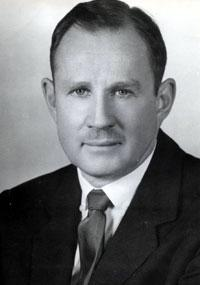
\includegraphics[scale=0.5]{../../../graphics/sellars.jpeg}
	\caption{Wilfrid Sellars}
	\label{fig:sellars}
\end{figure}

\section{An Ambiguity in Sense-Datum Theories} % (fold)
\label{sec:an_ambiguity_in_sense_datum_theories}

\textbf{Section 1}: Sellars aims to attack ``the whole idea of givenness,'' but proposes to do so by beginning with a special case---the given as it arises in sense-datum theories. Sellars doesn't explicitly tell us what the given is. No doubt he assumed that his audience at the University of London Special Lectures in Philosophy in March of 1956 knew, at least approximately, what he meant by the given. Whatever the merits of that assumption, it is less likely to be the case for us now. Instead, we must rely on the scattered clues provided by the text.

In attacking the given, Sellars doesn't mean to undermine the distinction between ``\emph{inferring} that something is the case and, for example, \emph{seeing} it to be the case''. Notice the distinction is between inferring and propositional seeing, seeing-\emph{that}. And since seeing is marked out as just an example, if a prominent one, the distinction is presumably between judgements formed on the basis of inference and non-inferential judgments paradigmatically (if not inevitably) formed on the basis of perception. ``The given'' is meant to carry ``substantial theoretical commitments'' that go beyond this commonplace.

\textbf{Section 2}: Sellars sketches the framework of the classical sense-datum theory. He focuses on the act--object structure that sense-datum theorists attribute to sensings understood as conscious episodes. On the one hand, there is the act of awareness or \emph{sensing}, and on the other hand there is the object of that awareness, the \emph{sense content}. Thus Moore in sensing the blue bead, we can distinguish the act of awareness---Moore's sensing, and what Moore was aware of---the sense content of that awareness (which presumably includes the bead's shape and color).

In addition, Sellars makes the suggestion that different sense modalities (visual sensing, tactual sensing, etc.) may be distinguished by their sense contents (as opposed to positing distinct kinds of sensings.) This is controversial given that there are sense contents available to distinct sensory modalities (we can see a shape and feel it).

\textbf{Section 3}: What's the ontological status of sense contents? Are they facts or particulars? This forms the basis of a dilemma:
\begin{enumerate}
	\item It is \emph{particulars} which are sensed. Sensing is not knowing. The existence of sense-data does not \emph{logically} imply the existence of knowledge.
	\item Sensing \emph{is} a form of knowing. It is \emph{facts} rather than \emph{particulars} which are sensed.
\end{enumerate}

The general suggestion is that there could be no mode of awareness that had the following two features:
\begin{enumerate}
    \item It is either a form of knowledge or entails that the subject of that awareness possesses knowledge of what they are aware
    \item The object of that awareness is a particular
\end{enumerate}
Notice so far in Sellars' discussion all that is in play of the sense-datum theory is the act--object structure of sensing and the (plausible if optional) hypothesis that the objects of sensings are particulars. Both claims can and have been endorsed by philosophers who are not themselves sense-datum theorists. One prominent historical example with which Sellars was undoubtedly familiar is early Prichard (at least prior to 1921 with ``Seeing Movements''). Early Prichard ascribes to \emph{perception} (if not experience) an act--object structure and insists that the objects of perception are particulars. So Sellars' dilemma for the sense-datum theorist is applicable to other positions as well. So not only is Russellian acquaintance a target here, but so is Cook-Wilsonian apprehension.

Sellars remarks that on the first alternative sensing a sense content (where sense contents are particulars) is a \emph{non-epistemic} fact. This is important since, as we shall see, the myth of the given is claimed to be analogous to Moore's naturalistic fallacy. Just as Moore claimed that it was a mistake to infer normative truths from (non-normative) natural truths, Sellars claims that it is a mistake to infer epistemic truths from non-epistemic truths. So what's an ``epistemic fact'' here? It is at least clear that facts about a subject's knowledge count as epistemic facts. So it is an epistemic fact about me that I know, say, that there was an earthquake in Haiti. Perhaps it is also the case that epistemic facts involve propositional states of a subject. But is the domain of epistemic fact broader than this? Suppose I justifiably believe that p, even if I fail to know that p. Would this count as an epistemic fact in Sellars sense? For the most part this won't matter since Sellars focus will be on the non-propositional character of sense data.

If we grant that ``the epistemological category of the given is, presumably, to explicate the idea that empirical knowledge rests on a `foundation' of non-inferential knowledge of matter of fact'', why is that in order for the given to play this epistemological role it must either \emph{be} or \emph{entail} non-inferential knowledge? Why must the sense in which the given \emph{grounds} non-inferential knowledge be wither identity or entailment (as opposed to some suitable explanatory relation)?

\textbf{Section 4}: Sellars suggests that the sense-datum theorist can have their cake and eat it to. The way to do so is to understanding sensing a particular in terms of having non-inferential knowledge of that particular. This will be logically coherent, but severs the thought that the given \emph{grounds} non-inferential knowledge.

Sellars considers some examples of the ordinary use of ``know'' that takes not a propositional complement but a noun phrase denoting a particular as a complement: ``Do you know John?'' (Putting aside controversial Rylean claims about knowing-how, one might also consider knowing-wh as a source of such examples, i.e., knowing-who, knowing-which, knowing-when, knowing-where). Is Sellars claiming that talk of knowledge here is just a \emph{façon de parler}? If so with what right?

\textbf{Section 5}: Sellars revisits an issue raised in section 2---whether or not sensing is analyzable. The first sentence of the paragraph is the major premise of the argument:
\begin{quote}
    We have seen that the fact that a sense content is a \emph{datum} (if, indeed, there are such facts) will logically imply that someone has non-inferential knowledge \emph{only} if to say that a sense content is given is contextually defined in terms of non-inferential knowledge of a fact about this sense content.
\end{quote}
If sensing is primitive or unanalyzable (and hence not so contextually defined), then there will be no such logical implication. Has the major premise really been established?

The second and third paragraphs raise the analogy between the myth of the given and Moore's naturalistic fallacy. The analogy is that just as normative facts cannot be reducible to (non-normative) naturalistic facts, so epistemic facts cannot be reducible to non-epistemic facts. Though Sellars clearly regards such reductionist ambitions to be a ``radical mistake'', he does not press this point here as it will be developed later in the argument. Is the analogy with Moore's naturalistic fallacy merely confined to anti-reductionism or is Sellars also implicitly emphasizing the normative character of epistemic facts?

\textbf{Section 6} Sellars claims that \emph{classical} (if not heterodox) sense-datum theorist are committed to an inconsistent triad of claims:
\begin{enumerate}
    \item \emph{X sense red sense content s} entails \emph{x non-inferentially knows that s is red}
    \item The ability to sense sense contents is unacquired
    \item The ability to know fact of the form \emph{x is Φ} is acquired
\end{enumerate}

\textbf{Section 7} Sellars provides a diagnosis of the difficulties encountered so far---``the classical concept of a sense datum [is] a mongrel resulting from a crossbreeding of two ideas''. Presumably this the ``ambiguity'' of the title of the present part:
\begin{enumerate}
    \item The idea that there are certain inner episodes---e.g. sensations of red or of C\# which can occur to human beings (and brutes) without any prior process of learning or concept formation; and without which it would \emph{in some sense} be impossible to \emph{see}, for example, that the facing surface of a physical object is red and triangular, or \emph{hear} that a certain physical sound is C\#.
    \item The idea that there are certain inner episodes which are the non-inferential knowings that certain items are, for example, red or C\#; and that these episodes are the necessary conditions of empirical knowledge as providing evidence for all other empirical propositions.
\end{enumerate}

% section an_ambiguity_in_sense_datum_theories (end)

\section{Another Language?} % (fold)
\label{sec:another_language_}

% section another_language_ (end)

\end{document}